\subsection{Software Architecture Requirements} \label{software_requirements}

Figure \ref{fig_design} illustrates the generic Software Architecture of the Artifacts.
Each instantiated element adheres to the Element Naming Convention outlined in Appendix
\ref{appendix_element_naming_convention}. In addition, the following tables detail the
requirements specific to each element.

\begin{figure}[H]
    \centering
    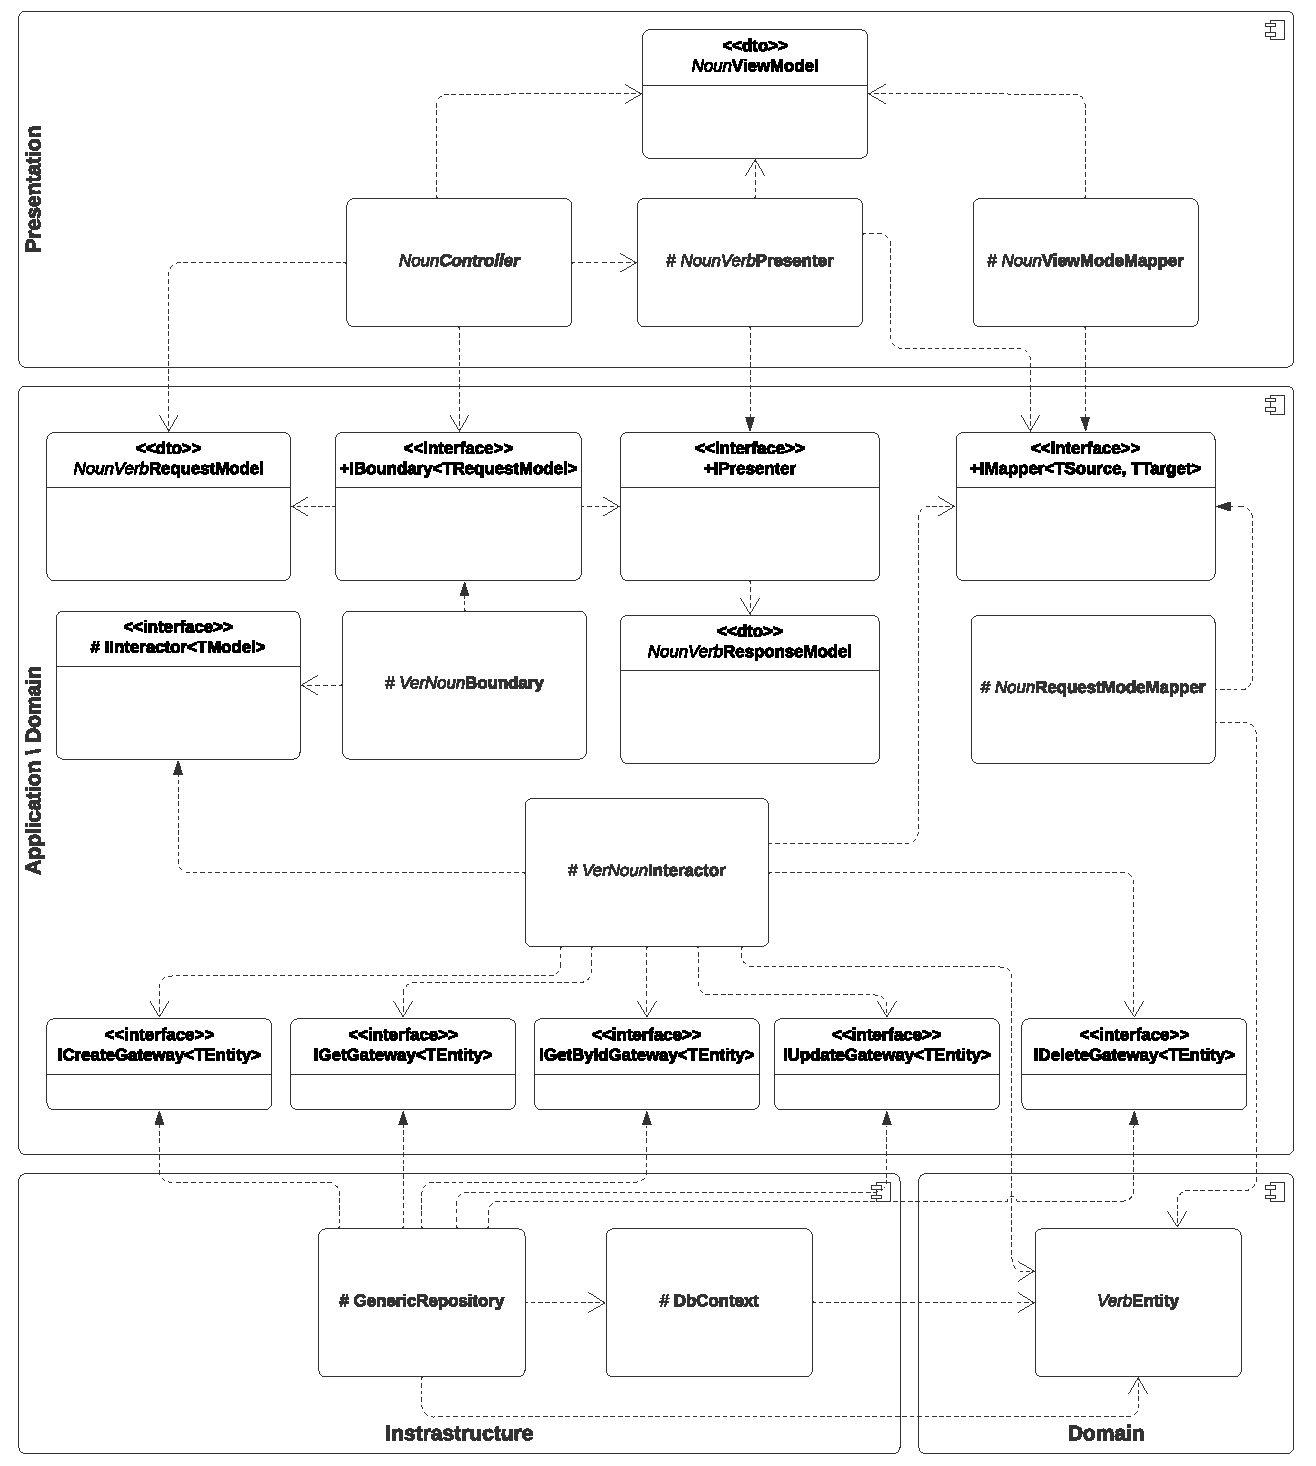
\includegraphics[width=1\textwidth]{figures/generic_design.pdf}
    \caption[Generic architecture]{The Generic architecture of the artifacts}
    \label{fig_design}
\end{figure}


\subsubsection*{Presentation Layer}
\begin{table}[H]
    \begin{tabular}{@{\makebox[2em][c]{\rownumber\space}}  p{0.87\linewidth}}
        \multicolumn{1}{@{\makebox[2em][c]{Nr.}}  p{0.87\linewidth}}{ViewModel Requirement}\\ 
        \hline
        The ViewModel consists of data attributes representing fields from the
        corresponding Entity. In addition, it may contain information specific to the user
        interface. \\

        The ViewModel has no external dependencies on other objects within the
        architecture. \\
       
       \hline
    \end{tabular}
\caption{ViewModel Requirements}
\label{table_requirements_viewmodel}
\end{table}

\begin{table}[H]
    \begin{tabular}{@{\makebox[2em][c]{\rownumber\space}}  p{0.87\linewidth}}
        \multicolumn{1}{@{\makebox[2em][c]{Nr.}}  p{0.87\linewidth}}{Presenter Requirement}\\ 
    \hline
    The Presenter Implementation is derived from the IPresenter interface and follows the
    specified implementation. The IPresenter interface can be found in the Application
    Layer. \\   
    
    The Presenter is responsible for creating the Controller's Response by instantiating
    the ViewModel, constructing the HTTP Response message, or combining both elements as
    needed. \\
    
    When required, the Presenter utilizes the IMapper interface without depending on
    specific implementations of the IMapper interface. \\
    
    The Presenter has an internal scope and cannot be instantiated outside of the
    Presentation layer. \\
    \hline
    \end{tabular}
\caption{Presenter Requirements}
\label{table_requirements_presenter}
\end{table}

\begin{table}[H]
    \begin{tabular}{@{\makebox[2em][c]{\rownumber\space}}  p{0.87\linewidth}}
        \multicolumn{1}{@{\makebox[2em][c]{Nr.}}  p{0.87\linewidth}}{ViewModelMapper Requirement}\\ 
    \hline
    The ViewModelMapper is derived from the IMapper interface and follows the specified
    implementation. The IMapper interface can be found in the Application Layer. \\

    The ViewModelMapper is responsible for mapping the values of the necessary data
    attributes from the ResponseModel to the ViewModel. \\
    
    The ViewModelMapper has an internal scope and cannot be instantiated outside of the
    Presentation layer. \\
    \hline
    \end{tabular}
\caption{ViewModelMapper Requirements}
\label{table_requirements_viewModelMapper}
\end{table}

\begin{table}[H]
    \begin{tabular}{@{\makebox[2em][c]{\rownumber\space}}  p{0.87\linewidth}}
        \multicolumn{1}{@{\makebox[2em][c]{Nr.}}  p{0.87\linewidth}}{Controller Requirement}\\ 
    \hline
    The Controller is responsible for receiving external requests and forwarding the
    request to the appropriate Boundary within the Application Layer. \\

    The Controller relies on the IBoundary interface without depending on specific
    implementations of the IBoundary interface. \\
    \hline
    \end{tabular}
\caption{Controller Requirements}
\label{table_requirements_controlle}
\end{table}

\subsubsection*{Application Layer}

\begin{table}[H]
    \begin{tabular}{@{\makebox[2em][c]{\rownumber\space}}  p{0.87\linewidth}}
        \multicolumn{1}{@{\makebox[2em][c]{Nr.}}  p{0.87\linewidth}}{IBoundary Requirements}\\ 
    \hline
    The IBoundary interface establishes the contract for its derived Boundary implementations. \\

    The IBoundary interface has public scope within the system. \\
    \hline
    \end{tabular}
\caption{IBoundary Requirements}
\label{table_requirements_iboundary}
\end{table}

\begin{table}[H]
    \begin{tabular}{@{\makebox[2em][c]{\rownumber\space}}  p{0.87\linewidth}}
        \multicolumn{1}{@{\makebox[2em][c]{Nr.}}  p{0.87\linewidth}}{Boundary Implementation Requirements}\\ 
    \hline
    A Boundary implementation is derived from the IBoundary interface and follows the
    specified implementation. \\

    The Boundary implementation serves as a separation between the internal aspects of the
    Application Layer and the other layers within the Component. \\
    
    Each Boundary implementation handles a single task, which is then
    executed using the IInteractor interface. \\
    
    Boundary implementations have an internal scope and cannot be instantiated outside the
    Application Layer. \\
    \hline
    \end{tabular}
\caption{Boundary Implementation Requirements}
\label{table_requirements_boundary}
\end{table}

\begin{table}[H]
    \begin{tabular}{@{\makebox[2em][c]{\rownumber\space}}  p{0.87\linewidth}}
        \multicolumn{1}{@{\makebox[2em][c]{Nr.}}  p{0.87\linewidth}}{IInteractor Requirements}\\ 
    \hline
    The IInteractor interface establishes the contract for its derived Interactor
    implementations. \\

    The IInteractor has an internal scope and cannot be implemented outside the Application
    Layer. \\
    \hline
    \end{tabular}
\caption{IInteractor Requirements}
\label{table_requirements_iinteractor}
\end{table}

\begin{table}[H]
    \begin{tabular}{@{\makebox[2em][c]{\rownumber\space}}  p{0.87\linewidth}}
        \multicolumn{1}{@{\makebox[2em][c]{Nr.}}  p{0.87\linewidth}}{Interactor Implementation Requirements}\\ 
    \hline
    An Interactor implementation is derived from the IInteractor interface and follows the
    specified implementation. \\

    The Interactor implementation executes a single task or orchestrates a series of
    tasks. Each of these tasks is implemented in separate Interactors. Alternatively, a
    Gateway is used for Tasks with Infrastructure dependencies, such as data persistence
    in a database. \\
    
    Depending on the Task, the Interactor implementation orchestrates the mapping from
    RequestModels to Entities, or from Entities to ResponseModels, utilizing the IMapper
    interface. \\
    
    Interactor implementations have an internal scope and cannot be implemented outside
    the Application Layer. \\
    \hline
    \end{tabular}
\caption{Interactor Implementation Requirements}
\label{table_requirements_interactor}
\end{table}

\begin{table}[H]
    \begin{tabular}{@{\makebox[2em][c]{\rownumber\space}}  p{0.87\linewidth}}
        \multicolumn{1}{@{\makebox[2em][c]{Nr.}}  p{0.87\linewidth}}{IMapper Requirements}\\ 
    \hline
    The IMapper interface establishes the contract for its derived Mapper implementations.
    \\

    The IMapper interface has a public scope within the system. \\
    \hline
    \end{tabular}
\caption{IMapper Requirements}
\label{table_requirements_imapper}
\end{table}

\begin{table}[H]
    \begin{tabular}{@{\makebox[2em][c]{\rownumber\space}}  p{0.87\linewidth}}
        \multicolumn{1}{@{\makebox[2em][c]{Nr.}}  p{0.87\linewidth}}{RequestModelMapper Requirement}\\ 
    \hline
    The RequestModelMapper is derived from the IMapper interface and follows the specified
    implementation. \\

    The RequestModelMapper is responsible for mapping the values of the necessary data
    attributes from the RequestModel to an Entity. \\
    
    The RequestModelMapper has an internal scope and cannot be implemented outside
    the Application Layer. \\
    \hline
    \end{tabular}
\caption{RequestModelMapper Requirements}
\label{table_requirements_requestmodelmapper}
\end{table}

\begin{table}[H]
    \begin{tabular}{@{\makebox[2em][c]{\rownumber\space}}  p{0.87\linewidth}}
        \multicolumn{1}{@{\makebox[2em][c]{Nr.}}  p{0.87\linewidth}}{ResponseModelMapper Requirement}\\ 
    \hline
    The RequestModelMapper is derived from the IMapper interface and follows the specified
    implementation. \\

    The RequestModelMapper is responsible for mapping the values of the necessary data
    attributes from the RequestModel to an Entity. \\
    
    The RequestModelMapper has an internal scope and cannot be implemented outside the
    Application Layer. \\
       \hline
    \end{tabular}
\caption{ResponseModelMapper Requirements}
\label{table_requirements_responsemodelmapper}
\end{table}

\begin{table}[H]
    \begin{tabular}{@{\makebox[2em][c]{\rownumber\space}}  p{0.87\linewidth}}
        \multicolumn{1}{@{\makebox[2em][c]{Nr.}}  p{0.87\linewidth}}{IPresenter Requirements}\\ 
    \hline
    The IPresenter interface establishes the contract for its derived Presenter
    implementations, typically implemented as part of the Presentation Layer. \\

    The IPresenter interface has a public scope within the system. \\
    \hline
    \end{tabular}
\caption{IPresenter Requirements}
\label{table_requirements_ipresenter}
\end{table}

\begin{table}[H]
    \begin{tabular}{@{\makebox[2em][c]{\rownumber\space}}  p{0.87\linewidth}}
        \multicolumn{1}{@{\makebox[2em][c]{Nr.}}  p{0.87\linewidth}}{I\textit{[\gls{verb}]}Gateway Requirements}\\ 
    \hline
    The \textit{[\gls{verb}]Gateway} interface establishes the contract for its derived Gateway
    implementations, which are typically implemented in the Infrastructure Layer. \\

    The \textit{[\gls{verb}]}Gateway interface has a public scope within the system. \\
    
    Each task is represented in the naming convention of the interface. As an example, the
    basic \gls{crud} actions result in a total of five IGateway interfaces: ICreateGateway,
    IGetGateway, IGetByIdGateway, IUpdateGateway, and IDeleteGateway. \\
    \hline
    \end{tabular}
\caption{\textit{[\gls{verb}]}Gateway Requirements}
\label{table_requirements_IGateway}
\end{table}

\begin{table}[H]
    \begin{tabular}{@{\makebox[2em][c]{\rownumber\space}}  p{0.87\linewidth}}
        \multicolumn{1}{@{\makebox[2em][c]{Nr.}}  p{0.87\linewidth}}{ResponseModel Requirement}\\ 
    \hline
    The ResponseModel consists primarily of data attributes representing the fields of the
    corresponding Entity. Additionally, the ResponseModel may contain data specific to the
    output of the Interactor. \\

    The ResponseModel does not depend on external objects within the architecture. \\
    \hline
    \end{tabular}
\caption{ResponseModel Requirements}
\label{table_requirements_responsemodel}
\end{table}

\begin{table}[H]
    \begin{tabular}{@{\makebox[2em][c]{\rownumber\space}}  p{0.87\linewidth}}
        \multicolumn{1}{@{\makebox[2em][c]{Nr.}}  p{0.87\linewidth}}{RequestModel Requirement}\\ 
    \hline
    The RequestModel consists primarily of data attributes representing the fields of the
    corresponding Entity. Additionally, the RequestModel may contain data specific to the
    input of the Interactor. \\

    The RequestModel does not depend on external objects within the architecture. \\
       
       \hline
    \end{tabular}
\caption{RequestModel Requirements}
\label{table_requirements_requestmodel}
\end{table}

\subsubsection*{Domain Layer}

\begin{table}[H]
    \begin{tabular}{@{\makebox[2em][c]{\rownumber\space}}  p{0.87\linewidth}}
        \multicolumn{1}{@{\makebox[2em][c]{Nr.}}  p{0.87\linewidth}}{Data Entity Requirement}\\ 
    \hline
    The Data Entity consists solely of attributes representing the corresponding data
    fields. \\

    The Data Entity does not rely on external objects within the architecture. \\
    
    The Application Layer is the only layer that utilizes the Data Entity. \\
    \hline
    \end{tabular}
\caption{RequestModel Requirements}
\label{table_requirements_requestmodel}
\end{table}

\subsubsection*{The Infrastructure Layer}

\begin{table}[H]
    \begin{tabular}{@{\makebox[2em][c]{\rownumber\space}}  p{0.87\linewidth}}
        \multicolumn{1}{@{\makebox[2em][c]{Nr.}}
        p{0.87\linewidth}}{\textit{[\gls{verb}]}Gateway Implementation Requirement}\\ 
    \hline
    The [\textit{\gls{verb}}]Gateway Implementation derives from the I[\textit{\gls{verb}}]Gateway interface
    and adheres to the specified implementation. \\

    The [\textit{\gls{verb}}]Gateway Implementation is responsible for the interaction
    associated with the specific task, utilizing the infrastructure technology of the
    specific layer (e.g., a SQL database or a filesystem).
    
    The [\textit{\gls{verb}}]Gateway Implementation has an internal scope and cannot be
    instantiated outside of the Layer. \\
    \hline
    \end{tabular}
\caption{\textit{[\gls{verb}]}Gateway Implementation Requirements}
\label{table_requirements_gatewayimplementation}
\end{table}

\subsubsection*{Design Principles compliancy}
Each architectural pattern adheres to at least one of the SOLID principles to ensure that
none of the implementations violate these principles.